\documentclass[12pt,a4paper,openright,twoside]{book}
\usepackage[utf8]{inputenc}
\usepackage{disi-thesis}
\usepackage{code-lstlistings}
\usepackage{notes}
\usepackage{shortcuts}
\usepackage{acronym}

\school{\unibo}
\programme{Corso di Laurea Magistrale in Ingegneria e Scienze Informatiche}
\title{Fancy Title}
\author{Francesco Magnani}
\date{\today}
\subject{Software Process Engineering}
\supervisor{Danilo Pianini}
\cosupervisor{Nicolas Farabegoli}
\morecosupervisor{Angela Cortecchia}
\session{III}
\academicyear{2023-2024}

% Definition of acronyms
\acrodef{IoT}{Internet of Thing}
\acrodef{vm}[VM]{Virtual Machine}
\acrodef{ide}[IDE]{Integrated Development Environment}
\acrodef{ci}[CI]{Continuous Integration}


\mainlinespacing{1.241} % line spacing in mainmatter, comment to default (1)

\begin{document}

\frontmatter\frontispiece

\begin{abstract}	
Max 2000 characters, strict.
\end{abstract}

\begin{dedication} % this is optional
Optional. Max a few lines.
\end{dedication}

%----------------------------------------------------------------------------------------
\tableofcontents   
\listoffigures     % (optional) comment if empty
\lstlistoflistings % (optional) comment if empty
%----------------------------------------------------------------------------------------

\mainmatter

%----------------------------------------------------------------------------------------
\chapter{Introduction}
\label{chap:introduction}
%----------------------------------------------------------------------------------------

Analyzing characteristics of the source code without necessarily building and executing it
(i.e., static analysis) is a process that has been studied and implemented in various 
forms during the last decades. Various tools have been developed to perform such a task, 
each with its own strengths and weaknesses.
%
The need for such a tool is often evident in the software development process, where ensuring the 
\textbf{quality} and \textbf{robustness} of software systems is a critical concern. Using 
code quality analysis techniques is also a powerful mean to avoid situations of 
``technical debt" \cite{DBLP:conf/sigsoft/ErnstBONG15}, that targets the system quality
in maintenance and evolution.
%
As the system grows in complexity, so does the variety of errors and vulnerabilities that can 
be detected through tools (e.g., concurrency management issues, error handling, etc.). 
At the same time, adhering to coding standards helps to avoid both trivial and non-trivial
errors from the outset. Additionally, these are among the easiest types of tools to integrate, 
often already included within \acp{ide}.
%
The effectiveness of static analysis tools has been the subject of various studies,  
\cite{DBLP:journals/jss/LenarduzziPSLP23} evaluating their detection capabilities, agreement, 
and precision. Some of these studies revealed a low degree of agreement among the tools and 
highlighted the need for a better understanding of their actual capabilities.  
%
In the last years, the static analysis tools have become more popular and easier to use, 
becoming protagonists of many \ac{ci} pipelines \cite{DBLP:conf/msr/ZampettiSOCP17} that 
automatically performs checks on the entire source code, embracing change and evolution of 
the software without making it a threat \cite{DBLP:books/daglib/0015650}, 
backed by a solid safety net.
%



% TO REMOVE
%----------------------------------------------------------------------------------------
Write your intro here.
\sidenote{Add sidenotes in this way. They are named after the author of the thesis}

For instance,
that you are discussing \acp{vm},
you may need both \ac{vm} and \acp{vm}.

\paragraph{Structure of the Thesis}

\note{At the end, describe the structure of the paper}




%----------------------------------------------------------------------------------------
\chapter{Background: the Collektive case}
\label{chap:background}
%----------------------------------------------------------------------------------------

I suggest referencing stuff as follows: \cref{fig:random-image} or \Cref{fig:random-image}

\begin{figure}
    \centering
    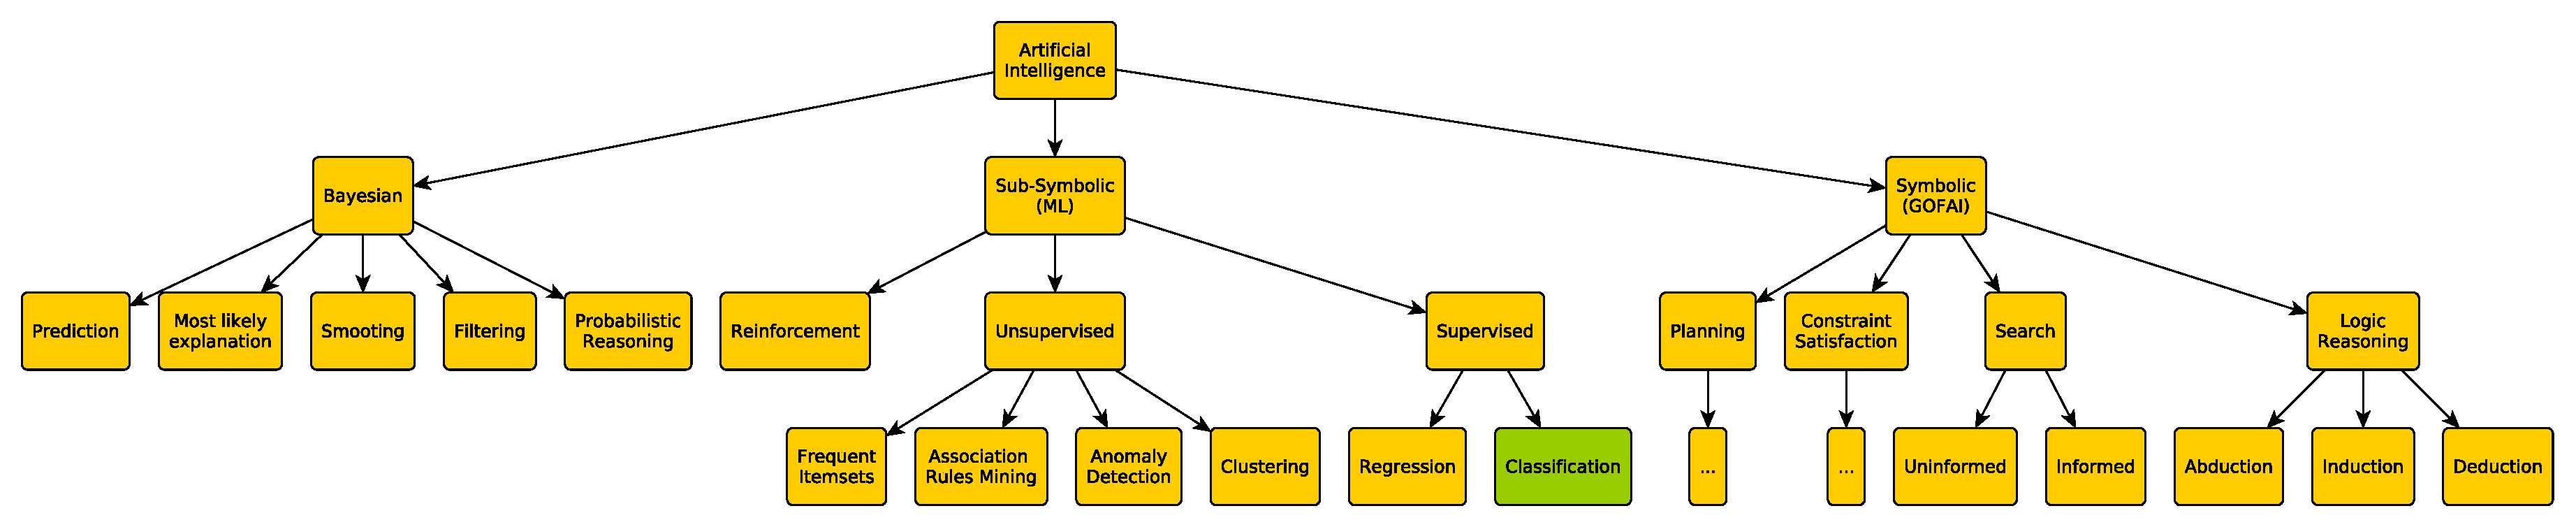
\includegraphics[width=.8\linewidth]{figures/random-image.pdf}
    \caption{Some random image}
    \label{fig:random-image}
\end{figure}

\section{Some cool topic}

%----------------------------------------------------------------------------------------
\chapter{Contribution}
\label{chap:contribution}
%----------------------------------------------------------------------------------------

You may also put some code snippet (which is NOT float by default), eg: \cref{lst:random-code}.

\lstinputlisting[float,language=Java,label={lst:random-code}]{listings/HelloWorld.java}

\section{Fancy formulas here}

%----------------------------------------------------------------------------------------
\chapter{Evaluation and Testing}
\label{chap:evaluation}
%----------------------------------------------------------------------------------------

%----------------------------------------------------------------------------------------
\chapter{Conclusion and Future works}
\label{chap:conclusion}
%----------------------------------------------------------------------------------------

%----------------------------------------------------------------------------------------
% BIBLIOGRAPHY
%----------------------------------------------------------------------------------------

\backmatter

\nocite{*} % Remove this as soon as you have the first citation

\bibliographystyle{alpha}
\bibliography{bibliography}

\begin{acknowledgements} % this is optional
Optional. Max 1 page.
\end{acknowledgements}

\end{document}
